% Pagina dei risultati

Una volta inserito il nome del locale da cercare nella barra di ricerca presente in Homepage (\S{8.1}) e cliccato sul bottone “Cerca”, all’utente verranno mostrati i risultati sotto forma di lista in una nuova pagina web, la quale conterrà il locale cercato (o i locali cercati, se ce ne sono più di uno con lo stesso nome) oppure, nel caso il locale non sia presente nel sistema, dei locali alternativi.

\begin{figure}[H]
\centering
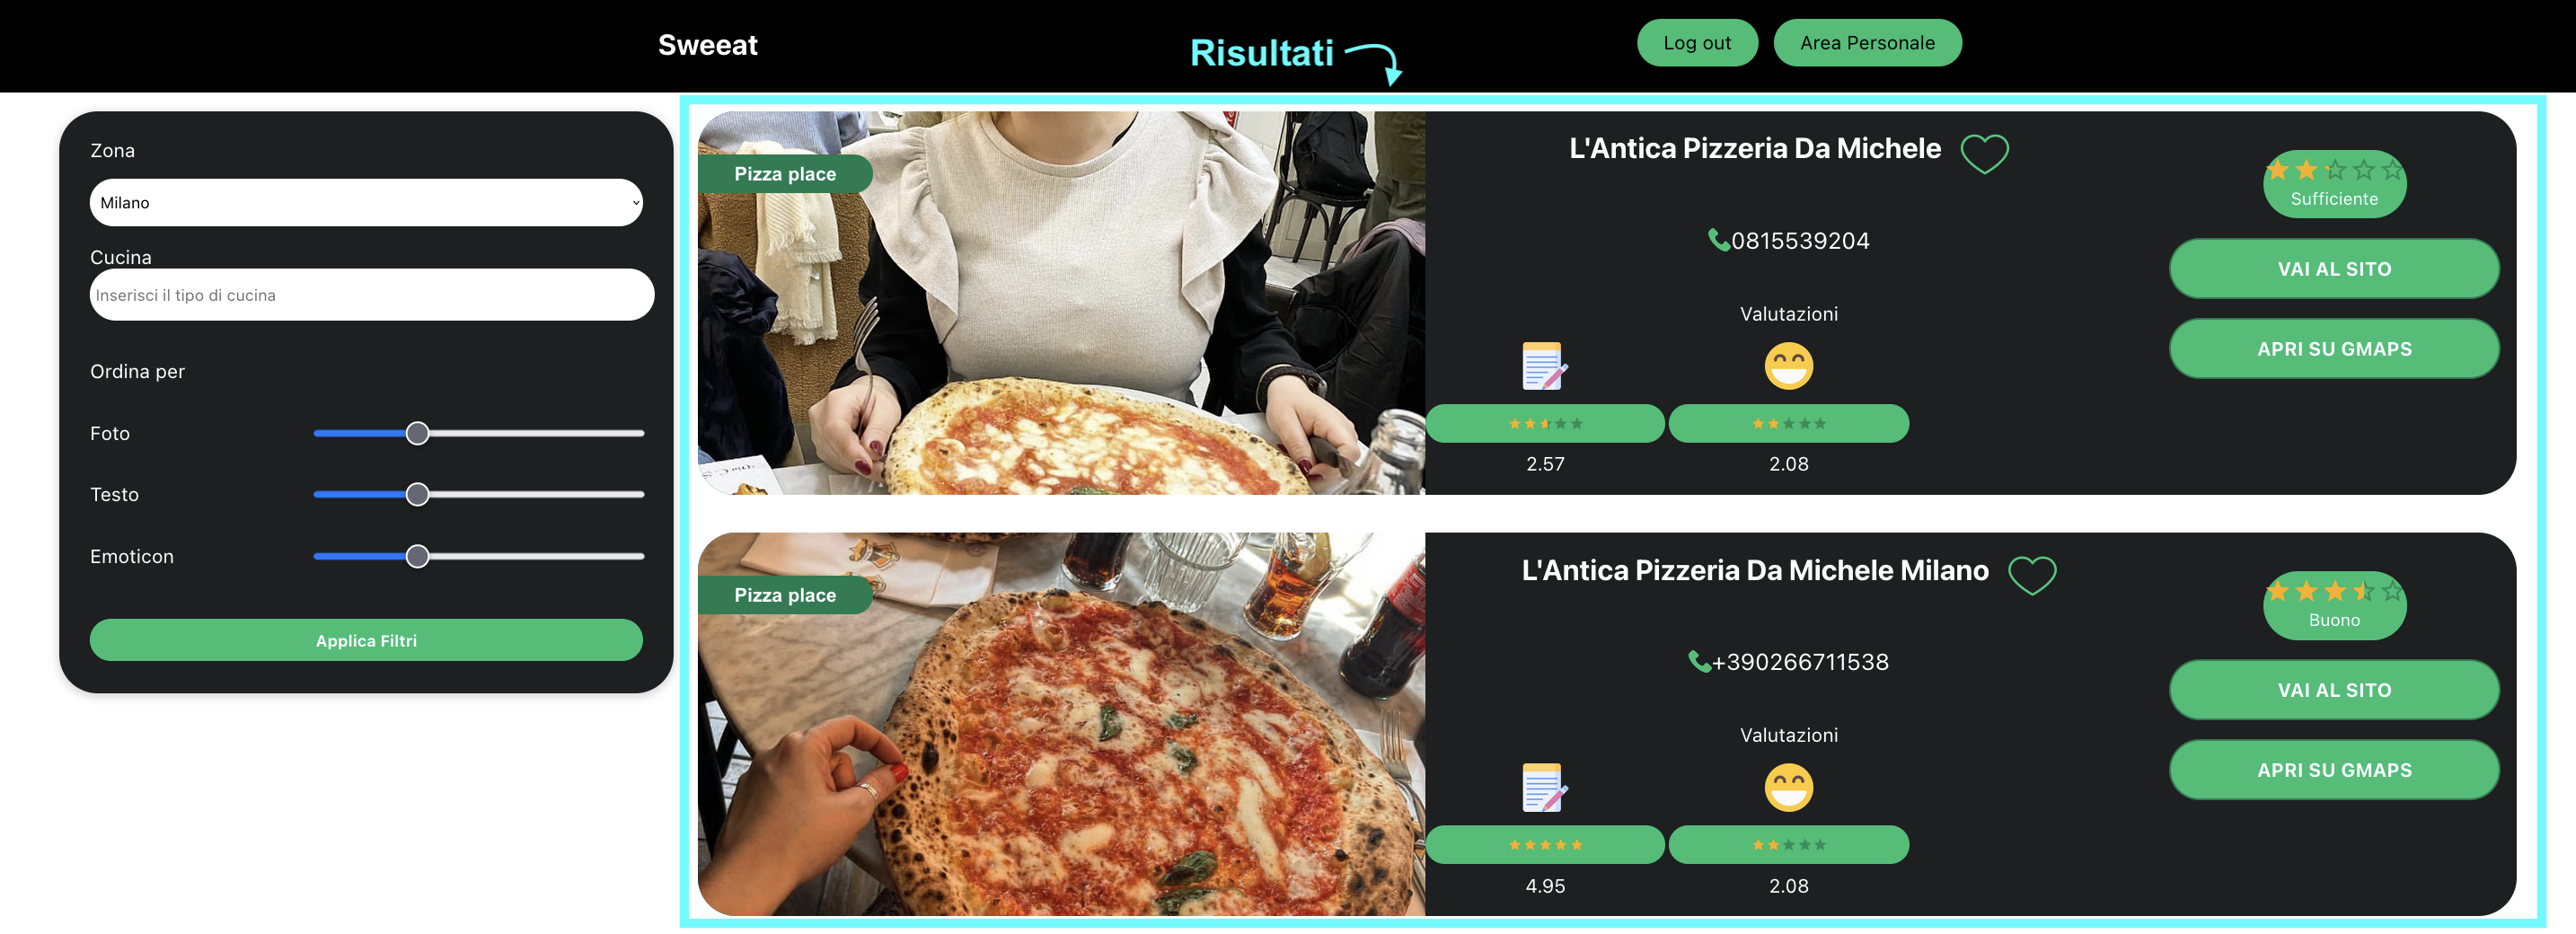
\includegraphics[scale=0.3]{./images/Ricerca/Ricerca.png} 
\caption{Pagina dei risultatati}
\end{figure}

I risultati mostreranno uno o più locali e, per ciascuno di essi, verranno mostrate le seguenti informazioni:

\begin{itemize}
\item Nome locale,
\item Valutazione complessiva,
\item Numero di telefono (opzionale),
\item Categoria,
\item Immagine di copertina del locale,
\item Valutazione per:
\begin{itemize}
\item Foto,
\item Testo,
\item Emoticon,
\end{itemize}
\item Link al sito web,
\item Link alla posizione del locale su Google Maps,
\item Possibilità di aggiungere o rimuovere il locale alla lista dei preferiti.
\end{itemize}

\begin{figure}[H]
\centering
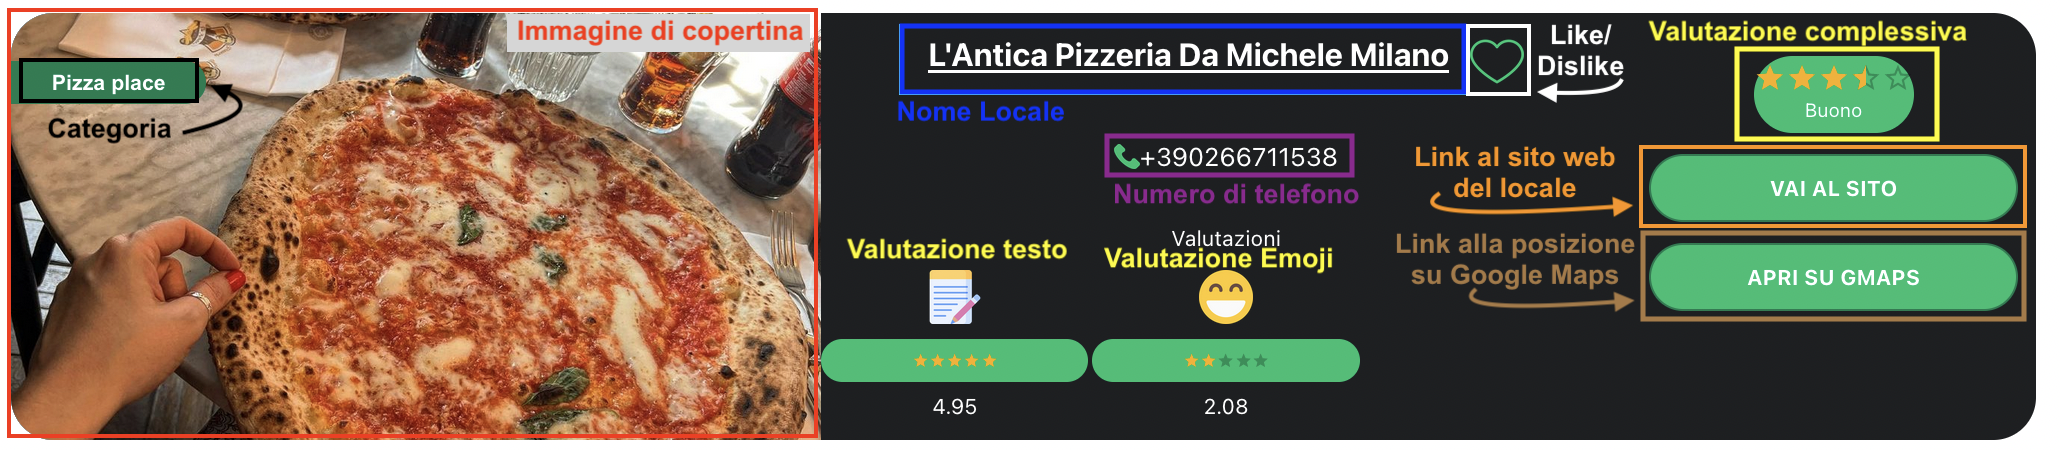
\includegraphics[scale=0.4]{./images/Ricerca/Card.png} 
\caption{Card locale nella pagina dei risultati}
\end{figure}

Inoltre, cliccando sul nome del locale all’utente verrà mostrata la pagina di dettaglio locale (\S{10}) la quale, oltre al nome del locale e le informazioni di base appena descritte, conterrà i contenuti multimediali relativi a quel locale pubblicati su Instagram ed utilizzati per realizzare la WebApp.

Nel caso la ricerca non vada a buon fine e non vengano trovati dei risultati, l’utente visualizzerà il seguente messaggio:

\begin{figure}[H]
\centering
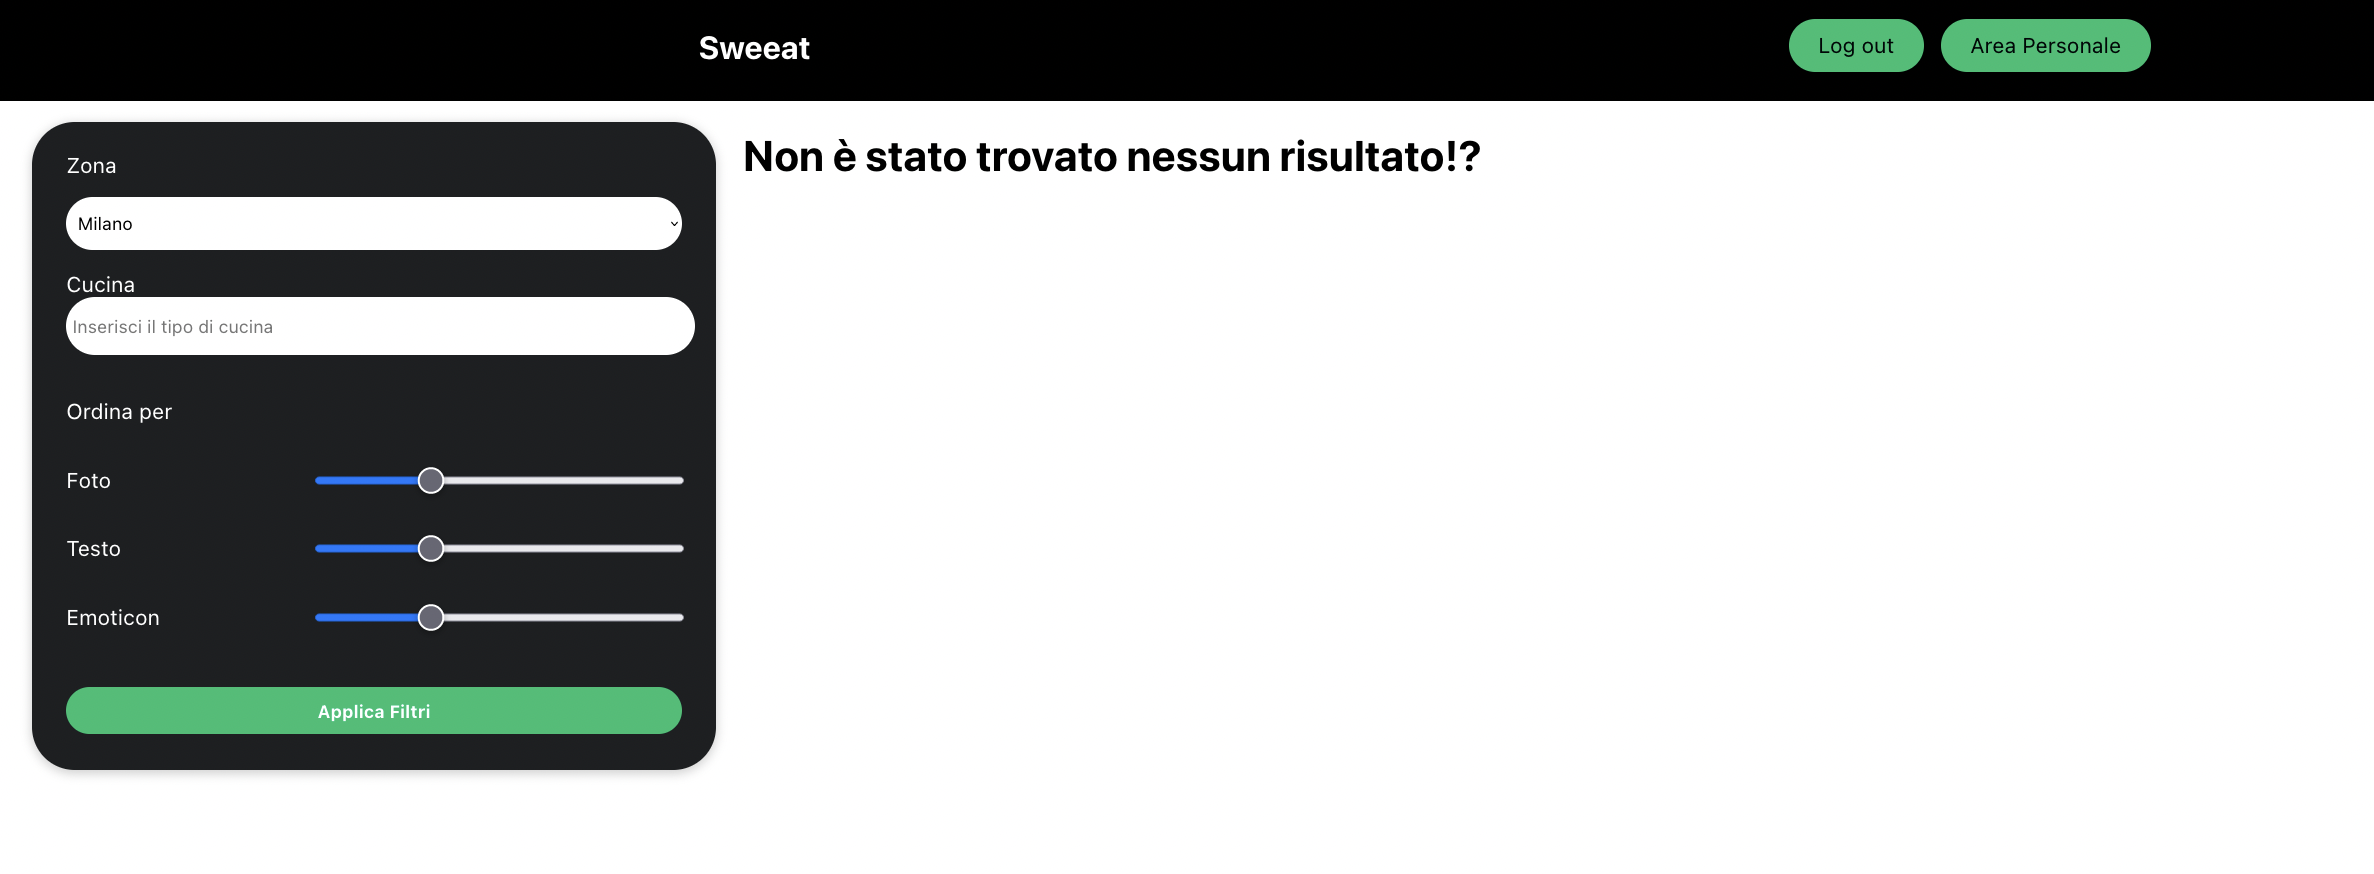
\includegraphics[scale=0.3]{./images/Ricerca/ZeroRisultati.png} 
\caption{Nessun risultato trovato per la ricerca}
\end{figure}

\subsection{Inserimento di un locale nella lista dei preferiti dalla classifica (solo per utenti registrati)}

Se l’utente ha effettuato il login (\S{5}) (tramite indirizzo e-mail e password), oltre alle informazioni di base del locale, accanto al nome del locale troverà l’icona a forma di cuore, che potrà essere:

\begin{itemize}
\item Rossa, se il locale è stato inserito nella lista dei preferiti (\S{7.4}),
\item Vuoto e con il bordo verde, nel caso in cui il locale non sia presente nella lista dei preferiti.
\end{itemize}

\begin{figure}[H]
\centering

\includegraphics[scale=0.6]{./images/Ricerca/Cuore.png} 
\caption{Inserimento/Rimozione locale nella lista dei preferiti}
\end{figure}

Un utente può inserire il locale nella propria lista dei preferiti semplicemente cliccando sopra al cuore vuoto con la cornice verde, mentre può rimuoverlo cliccando sul cuore rosso.

\subsection{Valutazioni}

Per ciascun locale presente nella piattaforma vengono mostrate le valutazioni di:

\begin{itemize}
\item Foto,
\item Testo,
\item Emoticon,
\item Valutazione complessiva.
\end{itemize}

Di base, la valutazione complessiva mostrata è data dalla somma delle valutazioni dei contenuti di foto, testo ed emoticon (in egual misura) di ciascun locale.

La valutazione complessiva delle foto è data dalle immagini pubblicate sui post Instagram e relative al locale in questione, analogamente viene svolto per testo (ossia, i testi dei post delle immagini) ed emoticon (ossia, il grado di soddisfazione del locale da parte dei volti che compaiono nelle immagini pubblicate sui post instagram).

\subsubsection{Il significato delle valutazioni}

Le valutazioni che esprimono la bontà del locale vengono espresse sotto forma di valore numerico ed il loro valore sarà compreso tra 1 e 5. Possiamo sintetizzare il significato del valore numerico come segue:

\begin{itemize}
\item \textbf{1}: pessimo-scarso,
\item \textbf{2}: scarso-sufficiente,
\item \textbf{3}: discreto-punteggio medio,
\item \textbf{4}: buono-ottimo,
\item \textbf{5}: ottimo-eccellente.
\end{itemize}

In sostanza, più il numero della valutazione si avvicina al “5”, migliore sarà la sua reputazione.


